\documentclass[thesis.tex]{subfiles}
\begin{document}
\chapter{Related Work}
\label{chap:related-work}
   
There has been relevant work on policy languages concurrent with our own work
capturing mobile security policies precisely. In this chapter we give an
overview of DKAL which built on SecPAL to describe how information could be
shared. We describe XACML an industrial standard for describing policies.
XACML was extended recently to describe delegation relationships. We explain
our reasons for choosing SecPAL as a basis for our work over it.

We also describe work developing fine-grained permissions systems for Android.
Policy languages give us a mechanism to describe trust relationships and
decisions \emph{in general}. Fine-grained permission systems are a type of
policy language to control app behavior on Android. To access some APIs, such as
access to private storage, Android apps must ask for a permission. Permissions
are a coarse usage control mechanism. Until 2015 (and Android Marshmallow),
users could not control which permissions an app had (by default).
Not installing an app was the only means to stop an app accessing data.
Android Marshmallow added the ability to disable many permissions of
an app after installation.

The coarseness of Android's permission system, and its relative inflexibility,
has led to a line of research into \emph{fine-grained} permissions systems.
These systems add extra permissions controls, and allow greater control of their
enforcement. We describe several notable examples and what extra controls
or new enforcement means the fine-grained permissions systems offered.

\section{DKAL}

The DKAL family of
languages~\cite{jeannin_dkal*:_2013,gurevich_dkal:_2008,yuri_gurevich_dkal2---simplified_2009}
grew from SecPAL as a policy language for a distributed
system's interacting agents~\cite{blass_introduction_2012}. Assertions are
communicated as signed statements called \emph{infons} between principals. For
example Alice might wish to recommend Bob an app. Alice, therefore, sends to Bob
the infon:

\begin{lstlisting}
alice said com.rovio.angrybirds is a good app.
\end{lstlisting}

Bob is free to do with this information as he wishes. He might accept app
recommendations from anyone and may have a rule to learn facts:

\begin{lstlisting}
with M: String, P: Principal
  upon
    P said M is a good app
  do
    learn P said M is a good app
\end{lstlisting}

DKAL2~\cite{yuri_gurevich_dkal2---simplified_2009} simplifies DKAL
language removing SecPAL's constructs for roles (the \emph{can-act-as} statement)
as Gurevich~\etal{} could not find a use for them in practice.  It also adds
support for sending infons if the recipient has completed an action:
for example only sending an app recommendation if the recipient has
asked for it.
DKAL\textsuperscript{$\star$}~\cite{jeannin_dkal*:_2013} took the ideas of information sharing
further and showed how to create executable protocols from DKAL programs.

DKAL improves over SecPAL by giving a means for transferring and reacting to
information. These might be helpful to describe how protocols worked within the
mobile ecosystem and for expanding how obligation policies would be triggered.
The authors of DKAL showed that all SecPAL policies could be expressed in
DKAL~\cite{gurevich_dkal:_2008}, so AppPAL could gain increased expressivity
just by switching interpretters.

\section{XACML}

XACML is a policy language with an industrial
standard~\cite{oasis_extensible_2013} that can be extended to fit many
scenarios. It is an attribute based policy language, but can also describe
role-based policies. It has tooling and enforcement infrastructure available
from Oracle. As a standard, it is important to summarize and briefly describe
why we chose to base our own work on SecPAL, a comparatively obscure policy
language, instead of the more well known XACML.

XACML policies are expressed as sets of \emph{rules} that describe whether a
specific action should be allowed or denied. When making a \emph{request} if a
rule's target matches it then the appropriate action should be taken. Rules are
combined into policies containing many rules which can contradict each other if
multiple ones match a given request. To handle contradictions a \emph{combining
algorithm} is used to decide how to proceed. Typical algorithms include:

\begin{description}
  \item[Permit-overrides.] If a rule gives a permit result then the request is permitted.
  \item[Deny-overrides.] If a rule gives a deny result then then the request is denied.
  \item[First-applicable.] The rules have an order of precedence. The first rule that gives a result decides the outcome.
  \item[Only-one-applicable.] Only one rule may match. If there are multiple matches an error is returned.
\end{description}

XACML's designers used natural language to describe the semantics of XACML. This
makes the semantics notoriously difficult to
interpret~\cite{ramli_detecting_2015}. There have been several attempts to
describe XACML's semantics
formally~\cite{ramli_xacml_2012,ramli_logic_2014,bryans_reasoning_2005}. Some of
these translations only describe a subset of XACML's
syntax~\cite{halpern_using_2008}. Others describe older versions of XACML which
are not compatible with the latest language versions~\cite{ahn_reasoning_2010},
Others have been found to contain mistakes caused by ambiguities in the
XACML specification~\cite{bruns_access-control_2008,halpern_using_2008}. All
these attempts help us understand XACML, but the lack of a single standard
semantics make it less attractive to extend to a new domain. As the language
grows and changes there are no present guarantees that any of the formal
semantics will remain correct and applicable to the current version of XACML. In
contrast, SecPAL's semantics are given precisely by
Becker~\cite{becker_secpal:_2006}.

Whilst SecPAL was designed for readability, XACML policies are verbose and
difficult to read. For example, to describe a simple policy that grants a principal,
\emph{Alice}, permission to do whatever she wants we might write:

\noindent\begin{minipage}{\linewidth}
\begin{lstlisting}
<xacml3:Policy xmlns:xacml3="urn:oasis:names:tc:xacml:3.0:core:schema:wd-17"
  PolicyId="http://axiomatics.com/alfa/identifier/alice.policy"
  RuleCombiningAlgId="urn:oasis:names:tc:xacml:3.0:rule-combining-algorithm:permit-overrides"
  Version="1.0">
  <xacml3:Description />
  <xacml3:PolicyDefaults>
    <xacml3:XPathVersion>http://www.w3.org/TR/1999/REC-xpath-19991116</xacml3:XPathVersion>
  </xacml3:PolicyDefaults>
  <xacml3:Target>
    <xacml3:AnyOf>
      <xacml3:AllOf>
        <xacml3:Match MatchId="urn:oasis:names:tc:xacml:1.0:function:string-equal">
          <xacml3:AttributeValue
            DataType="http://www.w3.org/2001/XMLSchema#string">alice</xacml3:AttributeValue>
          <xacml3:AttributeDesignator 
            AttributeId="urn:oasis:names:tc:xacml:1.0:subject:subject-id"
            DataType="http://www.w3.org/2001/XMLSchema#string"
            Category="urn:oasis:names:tc:xacml:1.0:subject-category:access-subject"
            MustBePresent="false"
          />
        </xacml3:Match>
      </xacml3:AllOf>
    </xacml3:AnyOf>
  </xacml3:Target>
  <xacml3:Rule 
      Effect="Permit"
      RuleId="http://axiomatics.com/alfa/identifier/alice.policy.Id_18">
    <xacml3:Description />
    <xacml3:Target />
  </xacml3:Rule>
</xacml3:Policy>
\end{lstlisting}
\end{minipage}

To help developers write policies, alternative notations are available that
compile into XACML's XML notation. ALFA is an alternate notation for
XACML~\cite{oasis_xacml_technical_comitee_abbreviated_2015} maintained by the
XACML developers. The equivalent ALFA policy of the above \emph{allow Alice all}
policy would be:

\noindent\begin{minipage}{\linewidth}
\begin{lstlisting}
namespace alice {
  policy policy {
    target clause Attributes.subjectId == "alice"
    apply permitOverrides
    rule {
      permit
    }
  }
}
\end{lstlisting}
\end{minipage}

The ALFA policy is more concise and shows the
policy's meaning more clearly than the XACML version.
There is an (Eclipse based) compiler for ALFA policies into
XACML~\cite{axiomaics_axiomatics_2012}, but there are not tools for
translating XACML to ALFA.  This means that any XACML policies would
need to be rewritten to take advantage of ALFA's syntax, and that any
tweaks made to a XACML policy cannot be trivially reintegrated into
the ALFA version.  Furthermore any analysis of XACML's semantics cannot
be trivially used to understand the semantics of ALFA.

Other notations exist including graphical
languages~\cite{henrik_nergaard_scratch-based_2015}, languages based on
propositional logic~\cite{zhang_synthesising_2004} and answer set
programming~\cite{ramli_xacml_2012}.

Whilst XACML 3.0 does support delegation~\cite{oasis_xacml_2010}, earlier
versions do not. The XACML 3.0 standard was published in 2013, after deciding to
start work with SecPAL. Despite XACML having a mechanism for delegation its
semantics, like the rest of the language, are poorly defined in natural
language. The standard gives one example of how delegation in XACML can be used:
a company has a printer and Carol is responsible for saying who can use the
printer. She delegates to Bob who in turn grants Alice the right to use the
printer. An excerpt from the XACML delegation policy example is shown in
\autoref{lst:xacml-deleg}. The full policy set is split into three smaller
policy\footnote{An individual decision in XACML is called a \emph{policy}, a
collection of policies is called a \emph{policy set}.}

\begin{figure}
  \begin{minipage}{1\textwidth}
    %\begin{multicols}{1}
      \lstinputlisting[basicstyle=\ttfamily\tiny,breaklines=true]{figures/xacmldelegation.xml}
    %\end{multicols}
  \end{minipage}
  \caption[Excerpt from XACML delegation example.]{Excerpt from XACML delegation example~\cite{oasis_xacml_2010}.}
  \label{lst:xacml-deleg}
\end{figure}

\begin{lstlisting}
'company' says 'carol' can-say inf
  Person:X canUse(Printer:P).

'carol' says 'bob' can-say
  Person:X canUse(Printer:P).

'bob' says 'alice' canUse(Printer:P).
\end{lstlisting}

Using ALFA we can also write delegation policies in the style of
XACML.  An example (taken from \cite{axiomatics_going_2016}) might be
a policy for a bank where only the account holder, or the account
holder's guardians can view their account:

\begin{lstlisting}
policy account{ 
  target clause object.objectType == "account"
  apply firstApplicable
  rule viewAccount{ 
    target clause action.actionId == "view"
    condition (user.username == account.owner) ||
      (stringIsIn(stringOneAndOnly(user.username),owner.guardians))
  }
}
\end{lstlisting}

The equivalent in AppPAL would be:

\begin{lstlisting}
'bank' says Person:O canView(Account:A)
if A hasOwner(O).

'bank' says Person:G canView(Account:A)
  if A hasOwner(O),
     O hasGuardian(G).

'bank' says Person:P can-say
  P hasGuardian(Person:G).
\end{lstlisting}

\begin{figure}
  \centering
  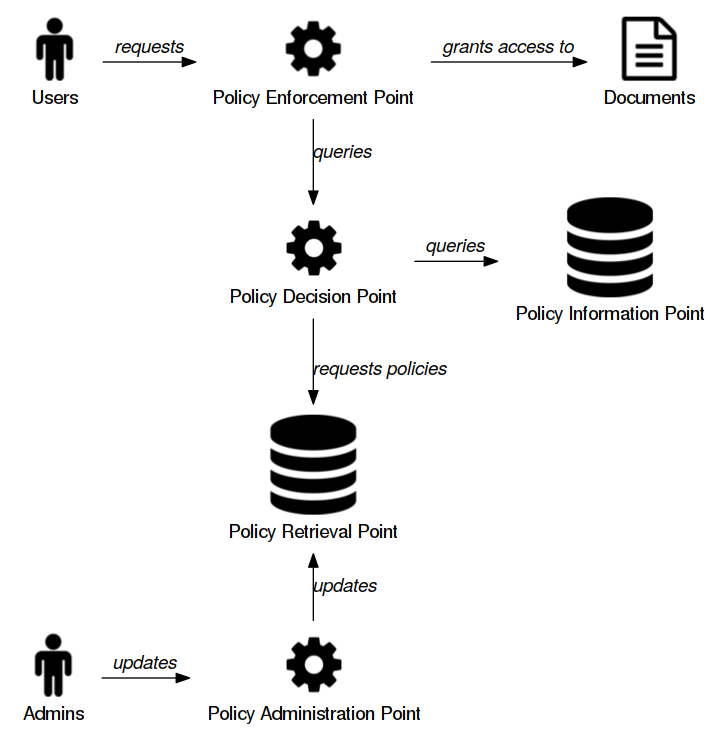
\includegraphics[width=0.6\textwidth]{figures/xacml-architecture.png}
  \caption{The XACML reference architecture.}
  \label{fig:xacml-architecture}
\end{figure}

XACML also defines a reference architecture for anyone seeking to use XACML,
shown in \autoref{fig:xacml-architecture}. The architecture consists of five
major \emph{policy points}: the PEP stands between the users and the files (for
example) they are trying to access. The PEP sends a query to the PDP (which
makes the \emph{decision}), and \emph{enforces} the policy by either granting or
denying access. In order to make the decision PDP \emph{requests} policies from
the PRP (which are updated by an \emph{administrator} editing the policies at
the PAP), and using \emph{information} from the PIP. 

XACML's architecture fits well with a centralized architecture, where
distributed PEPs talk to local PDPs which retrieve policies from a centralized
PRP. For a decentralized scenario the architecture fits less well as the
decision point may have to retrieve policies and decisions from multiple sources
(which may in turn require more decisions and policies to be retrieved).

Ultimately we chose to use SecPAL as the basis for our work instead of XACML as
it had well defined semantics, and was a better fit to describe the
decentralized policies of the mobile ecosystem. A lot of the results of our work
could have been replicated using XACML instead of AppPAL. Idioms found in BYOD
policies could be described in XACML as easily as they could in AppPAL. We could
have described app usage patterns using XACML and queried what apps they had
installed using that policy instead. But we used AppPAL as it felt a better fit.
Ultimately how we used the policy language is more interesting, we feel, than
which policy language we used.

\section{Fine-Grained Permission Systems}
\label{sec:fine-grained-permissions}

This section looks exclusively at Android as that is where the bulk of the
research has been. It is relevant to our work as these alternative permissions
schemes have been used to describe the policies about how users wish to use
their devices. The majority of the work has looked at Android: perhaps because,
unlike iOS, the operating system can be modified to incorporate new features.

The permission system of iOS allows users to
toggle an app's ability to perform certain actions (access photos,
send notifications) through the settings, and prompts users for a
default policy when the app first attempts to perform the action.
From Android Marshmallow the permissions schemes of iOS and Android
are very similar.

Some of the earliest work on fine-grained permissions systems for
Android starts with Enck~\etal's work on
Kirin~\cite{enck_lightweight_2009}.  Kirin allowed a user to define
what behavior they considered acceptable using a policy language.
Kirin ran on the device to certify apps using static analysis.  If an
app did not conform to the policy the user would be warned and could
uninstall it.  A natural next question is rather than rejecting the
entire app, can you just reject the behavior you don't like?
Ontang~\etal's SAINT tool~\cite{ongtang_semantically_2012} did just
that for inter-app communication, allowing the user to express a
policy about the circumstances two apps could share data or call
functionality.  Similarly Apex~\cite{nauman_apex:_2010} allowed user's
to specify at install time constraints as to when a permission could
be used.  
%This allowed them to write policies where an apps ability to send SMS messages
%could be denied if the app had already sent a message within the last hour, for
%example, or deny access to location data outside of working hours.
CRePE~\cite{conti_crepe:_2010} took
these ideas further allowing permissions to be denied based on
\emph{context} (for example the user was on a train, or the user was
within Bluetooth range of their computer).

Dr{.}~Android and Mr{.}~Hide~\cite{jeon_dr._2012} was a fine-grained permission
scheme that worked by rewriting apps to use guarded APIs.
AppGuard~\cite{backes_appguard_2013} worked similarly to Dr{.}~Android, but
allowed for controlled responses when a permission was denied---essentially
ensuring that the app didn't crash if it didn't get access to the data it
expected to. Aurasium~\cite{xu_aurasium:_2012} works by modifying apps to
monitor system calls and IPC mechanisms via GOT hijacking in the Bionic libc,
allowing their policies to effect native code which earlier tools ignored.

Jin~\etal{} developed a fine-grained permission system that targeted apps
written using the PhoneGap framework, that enable developers to create portable
native apps from web apps~\cite{jin_fine-grained_2015}. Dai~\etal{} proposed a
fine-grained permissions scheme that controlled apps (and IoT devices) access to
media stored on cloud based services based on a user's
policies~\cite{dai_who_2017}.

%SEAndroid was a set of patches to the Android kernel by the US
%National~Security~Agency porting the SELinux discretionary access
%control to Android~\cite{smalley_security_2013}.  The permissions
%system in Android had been implemented by using the Linux groups
%mechanisms.  When an app launched, the process would be created by
%forking a copy of the privileged \emph{zygote} Dalvik virtual machine
%process\footnote{A \emph{zygote} would run in the background permanently
%semi-initialised to allow apps to start quickly.}, which would then
%drop privileges and set gids based on the permissions the app declared.
%
%This implementation was problematic as it inherrited many of the
%problems with Linux's discretionary access control model, had no
%centralised policy document describing how permissions were used (the
%policy was expressed by the permissions of the filesystem), but also
%meant that the sandboxing mechanisms relied upon having this
%privileged zygote running (as well as potentially other services).
%
%SEAndroid ported the basic SELinux security mechanisms to Android,
%provided a default policy that described how the permissions and
%sandboxing systems should work under a mandatory access control
%scheme, and integrated it with the zygote system for starting
%apps.\footnote{SELinux policies are usually applied on
%\texttt{exec}-ing a process, not the \texttt{clone} used by the
%zygote.}
%
%Whilst SEAndroid did not implement a fine-grained permissions system
%by itself, it was merged into Android and would replace the original
%permissions system.  By Android Marshmallow it was fully enabled, and
%allowed an app's permissions to be granted or denied by the user as
%the permissions system was far more flexible than the original DAC
%implementation.


\end{document}

%%% Local Variables:
%%% mode: latex
%%% TeX-master: "../ch7.tex"
%%% End:
